% INTRODUCTION
\begin{tframe}{Introduction}

\vspace{0.2cm}

In an increasingly digital world, the analysis of multimedia objects is rapidly assuming importance in the context of digital investigation.

\vspace{0.5cm}

Multimedia Forensics has developed many techniques with the goal of providing aid in making decisions about a digital content authenticity, integrity and origin.

\begin{figure}
\centering
    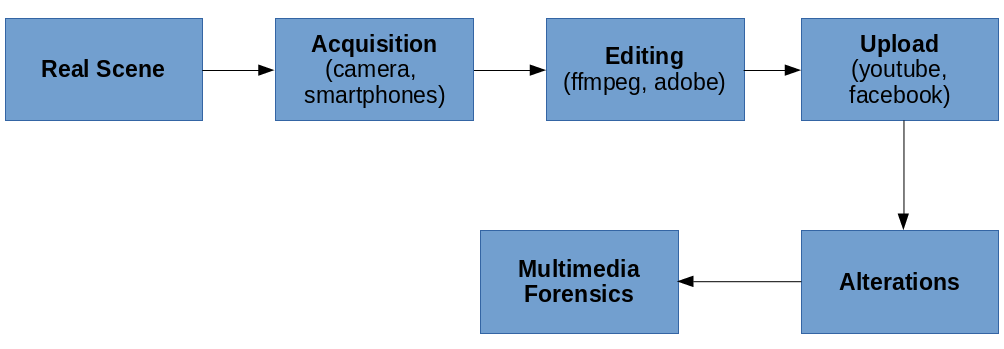
\includegraphics[width=0.85\textwidth]{images/workflow.png}
\end{figure}

\end{tframe}

% INTRODUCTION
\begin{tframe}{Introduction}

\vspace{0.2cm}

We have focused our attention on Source Identification and Integrity Verification of digital videos acquired by smartphones and tablets.

\vspace{0.5cm}

In this regard, techniques mainly use two different tools:

\begin{enumerate}
\item \textbf{Audio-video signal}: the research of inconsistencies and artefacts in the digital content.
\item \textbf{Metadata}: the determination of their compatibility, completeness, and consistency.
\end{enumerate}

\end{tframe}

% FILE CONTAINERS - WHAT'S INSIDE
\begin{tframe}{Video File Container - What's inside?}

\vspace{0.2cm}

\begin{minipage}{\textwidth}
\begin{columns}[T]

\begin{column}{0.55\textwidth}
\textbf{Container data}, structured information about the content, like:
\begin{itemize}
\item Content-related metadata (acquisition time, place, settings, etc.)
\item Number of tracks/signals (e.g. a video container may include several video tracks.)
\end{itemize}

\textbf{Codec data}, necessary information to decode and present the signal, like:
\begin{itemize}
\item Quantization tables.
\item Information for entropy decoding
\end{itemize}

\textbf{Encoded signal(s)}
\end{column}

\begin{column}{0.45\textwidth}
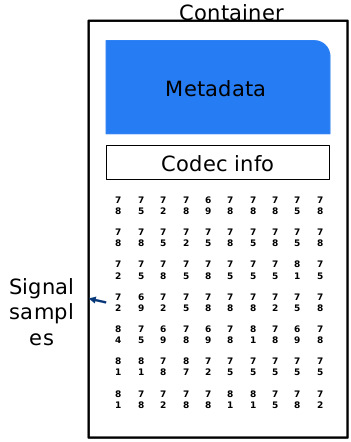
\includegraphics[width=1\textwidth]{images/container.png}
\end{column}

\end{columns}
\end{minipage}

\end{tframe}

% FILE CONTAINER - STRUCTURE
\begin{tframe}{Video File Container - Structure}

\vspace{0.5cm}

\begin{minipage}{\textwidth}
\begin{columns}[T]

\begin{column}{0.55\textwidth}

As defined by the \emph{ISO Base Media File Format Standard} [1], file containers have a object-oriented type structure.

\vspace{0.5cm}

Each object, called \emph{box} or \emph{atom}, includes specifics information about the media and are identified by 4-byte characters (e.g. \emph{ftyp}, \emph{mdat}, \emph{moov}, etc.).

\vspace{0.5cm}

Boxes can have fields and can contain other boxes.

\end{column}

\begin{column}{0.45\textwidth}
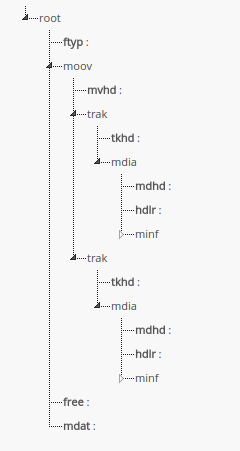
\includegraphics[width=0.75\textwidth]{images/tree.png}
\end{column}

\end{columns}
\end{minipage}

\end{tframe}

% FILE CONTAINER - WHY
\begin{tframe}{Video File Container - Why?}

\uncover<1->{As noticed by \emph{Gloe et al.} [2], the video format standards (e.g. \emph{ISO Base Media} [1], \emph{MP4} [3], \emph{MOV} [4]) for the file container prescribe only a limited number of features.}

\uncover<2->{
$$\Downarrow$$
Freedom of interpretation for the device manufacturers in terms of design decisions (order of the boxes, attributes values, etc.).
}

\uncover<3->{
$$\Downarrow$$
Low-level information to be exploited by the Forensic Analyst.
}

\end{tframe}

% SOURCE IDENTIFICATION
\begin{tframe}{Source Identification}

\vspace{0.1cm}

Given a video, we want to assess its origin based on its file container.

\vspace{0.5cm}

We split the problem in binary questions.

\vspace{0.5cm}

Ex. Does the video belongs to Samsung? \newline
	 ... to Samsung Galaxy S3? \newline
	 ... to Huawei G6? \newline
	 ... to Apple? \newline
	 ... to Apple iPhone 5? \newline
	 
\vspace{0.1cm}

Given a question, a training dataset is queried to obtain two classes (videos for which the answer is true, and the complementary).

\vspace{0.5cm}

For each question, we want to define a compatibility score.

\end{tframe}

% TRAINING
\begin{tframe}{Source Identification - Training}

\vspace{0.1cm}

Determine whether a video belongs to a class $C$ (e.g. Samsung).

\vspace{0.1cm}

We split the ground-truth in two sets:

$$ \Omega = X_{C} \cup X_{\overline{C}} = {x_{1}, \ldots, x_{N_{C}} \in C} \cup {x_{1}, \ldots, x_{N_{\overline{C}}} \in \overline{C}} $$

$\Omega$ contains all the attributes $\omega$ of the boxes contained in each of the ground-truth media.

\vspace{0.5cm}

We determine the discrimination power of each of the attributes $\omega$ for the class $C$ and $\overline{C}$.

\begin{minipage}{\textwidth}
\begin{columns}[T]

\begin{column}{0.45\textwidth}
$$  W_{C}(\omega) = \dfrac{\sum\limits_{i=1}^{N_{C}}\mid X_{i} \cap \omega \mid}{N_{C}} $$
\end{column}

\begin{column}{0.45\textwidth}
$$  W_{\overline{C}}(\omega) = \dfrac{\sum\limits_{i=1}^{N_{\overline{C}}}\mid X_{i} \cap \omega \mid}{N_{\overline{C}}} $$
\end{column}

\end{columns}
\end{minipage}

\end{tframe}

% TEST
\begin{tframe}{Source Identification - Test}

Given a media query $X = \omega_{1}, . . . \omega_{t}$, we solve the two hypothesis test problem:

$$  H_{0}:X \in \overline{C} $$
$$  H_{1}:X \in C $$

To do so, we determine the likelihood ratio of observing $\omega_{j}, j = 1 \ldots t$.

\vspace{1cm}

\begin{minipage}{\textwidth}
\begin{columns}[T]

\begin{column}{0.45\textwidth}
$$ P(\omega_{j}\vert H_{0}) = W_{\overline{C}}(\omega_{j}) $$
$$ P(\omega_{j}\vert H_{1}) = W_{C}(\omega_{j}) $$ 
\end{column}

\begin{column}{0.45\textwidth}
$$ L(X) = \prod\limits_{\omega_{j}}\dfrac{W_{C}(\omega_{j}) }{W_{\overline{C}}(\omega_{j})} $$
\end{column}

\end{columns}
\end{minipage}

\vspace{0.5cm}

Then, $l(X) = lnL(X)$ can be used to determine whether $X$ belongs to class $C$.

\end{tframe}

% ENTROPY
\begin{tframe}{Source Identification - Correlated Features}

Some features might be correlated. For each box, we consider the entropy of its attributes in order to remove redundant information.

\vspace{0.1cm}

When considering a box, given a vector of likelihood ratios $\overline{x} = (x_{1},\ldots,x_{n})$, we compute the likelihood for that box as:

$$ L(\overline{x}) = \prod\limits_{i=1}^{n} x_{i}^{\alpha_{i}} $$ with $$ \alpha_{i} = \dfrac{(n-1)\gamma_{i}+1}{n} $$ $$ \gamma_{i} = - \dfrac{n}{log n} P(x_{i})log P(x_{i}) $$ and where $P(x_{i})$ represents the probability of finding that value of ratio in the vector.

\end{tframe}

\begin{tframe}{Source Identification - Experiments}
The dataset is composed of 260 videos acquired from smartphones and tablets with Android (Samsung, Huawei) and iOS.
\vspace{0.2cm}

The tests are divided in two types, changing the definition of a class of device:

\begin{itemize}
\item \textbf{Brand}: we try to identify the test videos brand (3 brands).
\vspace{0.1cm}
\item \textbf{Model}: we try to identify both brand and model (13 models).
\end{itemize}
\vspace{0.2cm}

For each of these types, we consider:

\begin{itemize}
\item \textbf{Binary Classification}: for each class of devices in the dataset, we try to correctly classify the test videos.
\vspace{0.1cm}
\item \textbf{Retrieval}: how many times the correct classes are in the first position, in the top three position, or in the top five position (ordered by the likelihood ratios).
\end{itemize}

\end{tframe}

\begin{tframe}{Source Identification - Results}

\begin{footnotesize}
\begin{table}[h!]
\centering
\begin{tabular}{c c c c c c c} 
\hline \hline 
\textbf{Type} & \textbf{ACC} & \textbf{THRESHOLDS} & \textbf{TH = 0} & \textbf{TOP 1} & \textbf{TOP 3} & \textbf{TOP 5}\\ [0.5ex]
\hline

Brand & 98.08\% & [-12, 14] & 98.08\% & 92\% & - & - \\
Model & 97.54\% & [3, 4] & 96.79\% & 84.62\% & 100\% & 100\% \\

\hline
\end{tabular}
\end{table}
\end{footnotesize}

\vspace{0.1cm}
    
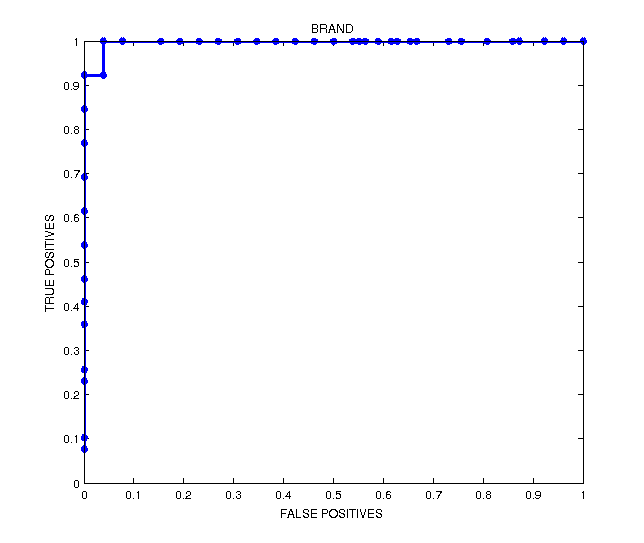
\includegraphics[width=0.5\textwidth]{images/brand-plot-label.png}
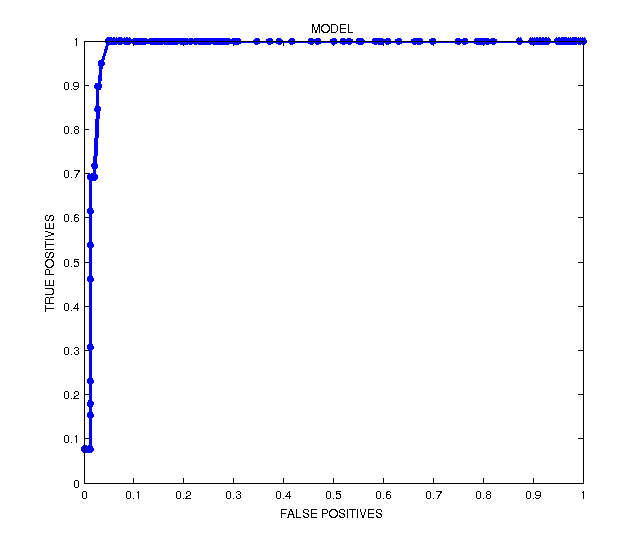
\includegraphics[width=0.5\textwidth]{images/model-plot-label.png}

\end{tframe}

\begin{tframe}{Integrity Verification}

\vspace{0.2cm}
\uncover<1->{Given a query video $X$ that supposedly comes from a certain device.
}


\uncover<2->{
$$\Downarrow$$
We want to assess if this supposition is true or if the video has been altered in some way.
}


\uncover<3->{
$$\Downarrow$$
We obtain a reference video $Y$, acquired by the supposed device.
}


\uncover<4->{
$$\Downarrow$$
By comparing the two file containers, we compute the percentage of differences.
}

\end{tframe}

\begin{tframe}{Integrity Verification - Experiments}

For these experiments, we have altered the videos of the dataset with different tools:

\begin{itemize}
\item \textbf{Ffmpeg}: we have directly cut the videos, without re-encoding.
\vspace{0.1cm}
\item \textbf{Exiftool}: we have changed the metadata related to Date and Time.
\vspace{0.1cm}
\item \textbf{YouTube}: we have uploaded and downloaded the videos from \emph{YouTube}.
\end{itemize}

\vspace{0.5cm}

Using their file containers, we compute the differences:

\begin{enumerate}

\item $(x_{1},\ldots,x_{n}) \in C_{i}$, $(x_{i}, x{j}) \rightarrow d_{ij}$
\vspace{0.1cm}
\item $(\overline{x_{1}},\ldots,\overline{x_{n}}) \in \overline{C_{i}}$, $(x_{i}$, $\overline{x_{j}}) \rightarrow \overline{d_{ij}}$ 
%and $(\overline{x_{i}}, x_{j}) \rightarrow \overline{d_{ji}}$

\end{enumerate}

\end{tframe}

\begin{tframe}{Integrity Verification - Results}

\begin{footnotesize}
\begin{table}[h!]
\centering
\begin{tabular}{l c c c c c c c} 
\hline \hline 
\textbf{N.} & \textbf{Tool} & \textbf{ACC} & \textbf{THRESHOLD}\\ [0.5ex]
\hline
1 & Ffmpeg & 100\% & [0.11, 0.66]\\
2 & Exiftool & 100\% &	0.001 \\
3 &	YouTube & 100\% & [0.39, 0.55] \\ 

\hline
\end{tabular}
\end{table}
\end{footnotesize}

\vspace{0.2cm}
Using the file containers, we were always able to correctly separate the original videos from the modified ones.

\vspace{0.5cm}
For the \emph{Exiftool} case, we did not consider the differences caused by attributes whose values are unique to each video (acquisition time, modification time, duration, size, etc.).

\end{tframe}

\begin{tframe}{Integrity Verification - Results}

\begin{figure}
\centering
    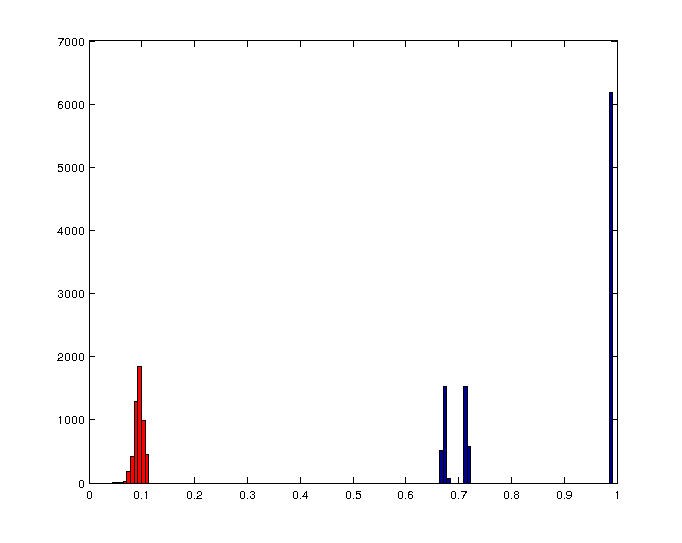
\includegraphics[width=0.70\textwidth]{images/ffmpeg-hist.png}
    \caption{Differences distribution for the Ffmpeg case. Red for original videos; blue for modified videos.}
\end{figure}

\end{tframe}

\begin{tframe}{Web Application}

\begin{figure}
\centering
    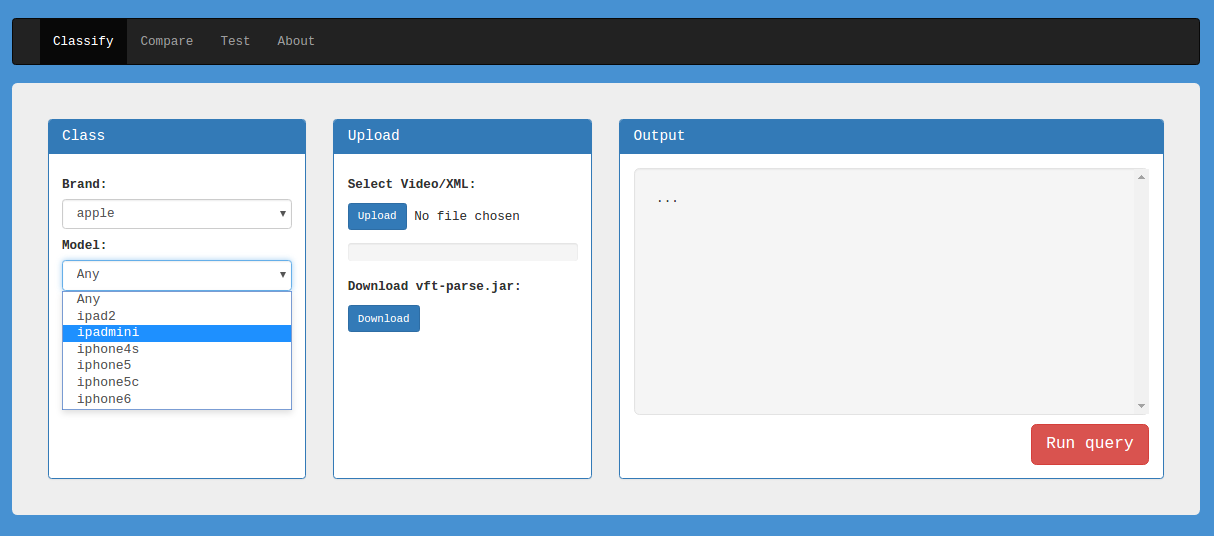
\includegraphics[width=1\textwidth]{images/webapp.png}
    \caption{Interface for the Source Identification feature.}
\end{figure}

\end{tframe}

\begin{tframe}{Conclusions}

\begin{itemize}
\item Using the video file containers, we implemented two approaches for Source Identification and Integrity Verification.
\vspace{0.1cm}
\item Video file container turned out to be a powerful tool; both approaches achieved promising results.
\vspace{0.1cm}
\item Should be considered preliminary work; further developments:
\begin{itemize}
\vspace{0.1cm}
\item Perform tests with a higher variety of devices.
\vspace{0.1cm}
\item Take into consideration the version of the operating system.
\vspace{0.1cm}
\item Specialize how the attributes are compared (e.g. check for format for Date and Time).
\vspace{0.1cm}
\item For Source Identification, it is critical how the reference population is built.
\end{itemize}
\end{itemize}
\end{tframe}
